% !TEX root = Calli.tex

\section{Programmstruktur / Methodik}
\label{sec:Programmstruktur}

Zum Lösen der Aufgabe wird die Programmiersprache \emph{Python 2.7} verwendet. In Form der Open-Source Library \emph{OpenCV} steht dazu eine leistungsstarke Bibliothek zur Bildverarbeitung zur Verfügung.
OpenCV selbst ist in C++ geschrieben, bietet jedoch entsprechende Python-Bindings an.


\subsection{Vorgehensweise}

Favorisiert wird eine extern angeschlossene Webcam angesprochen. Findet die Software keine Kamera, so greift sie auf die interne Kamera des Computers zurück. 

\lstset{language=Python}
\begin{lstlisting}[]
# create video capture
# try external Webcam
try: cap = cv2.VideoCapture(1)
# except internal Webcam
except:  cap = cv2.VideoCapture(0)
\end{lstlisting}

\subsection{Farbsegmentierung}

Das Ausgangsbild wird zunächst nach Farben gefiltert. Dabei entstehen Binärbilder für jede Farbe / Frucht. 

\begin{figure}[h]
    \centering
    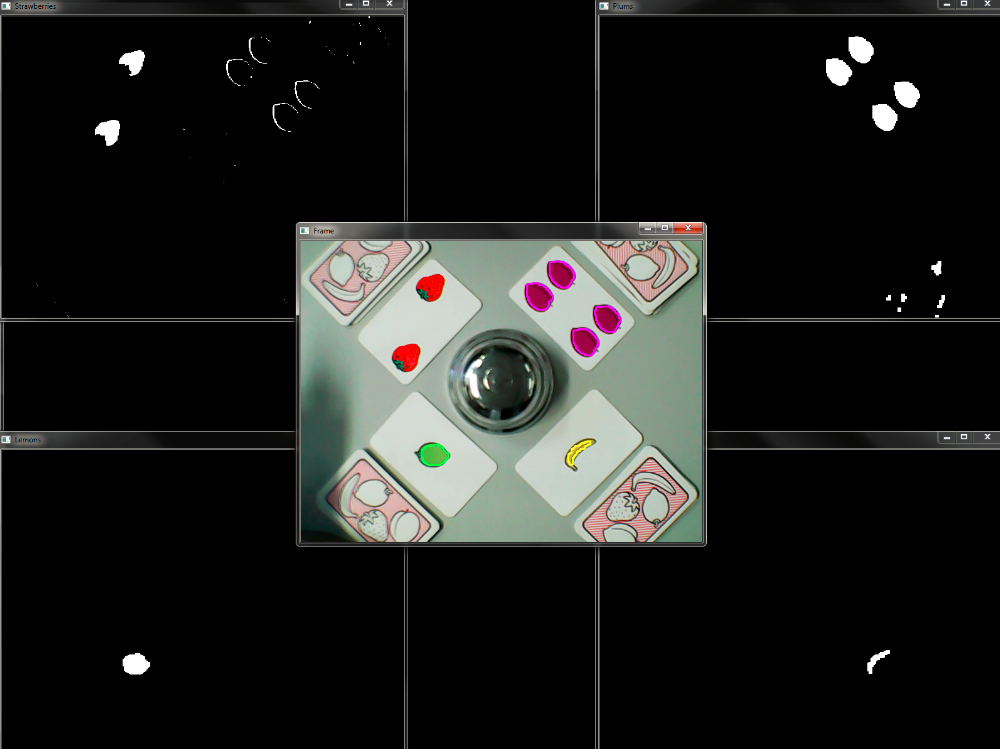
\includegraphics[width=10cm]{Abbildungen/Binaerbild01}
    \caption[Binär01]{Beispielbild mit Binärbildern für jede Frucht}
    \label{fig:Binär01}
\end{figure}

\subsubsection{HSV-Raum}

Um die einzelnen Früchte sicher detektieren zu können, wird zuerst das Ausgangsbild gefiltert und in den HSV-Raum übertragen. Die Farben werden einzeln extrahiert. Jede Farbe wird mit Hilfe des Farbwertes (Hue - Wert ), der Farbsättigung (saturation) und der Dunkelstufe / des Hellwertes (value) definiert. Die Beschreibung der Parameter erfolgt in folgenden Bereichen:

\textbf{Farbwert} Farbwinkel auf dem Farbkreis (z.B. 0 $^\circ$ für rot) - Bereich OpenCV [0,179]

\textbf{Farbsättigung} Sättigung in Prozent (z.B. 0\% Neutralgrau) - Bereich OpenCV [0,255]

\textbf{Hellwert} Helligkeit in Prozent (z.B.100\% volle Helligkeit) - Bereich OpenCV [0,255]

Minimum - und Maximumwert für die Farbbereiche der Früchte können zur Kalibrierung über Schieberegler eingestellt werden. Abhängig von der Beleuchtung und der verwendeten Kamera variieren diese, sodass eine Anpassung zum Beginn des Prozesses sinnvoll ist. 

Für die Farben der Früchte des Halli Galli Spiels ist der HSV-Raum fest definiert. Die Bereiche zur Filterung werden entsprechend darum festgelegt. 

\begin{itemize}
    \item Limone - hellgrün - HSV(93, 64\%, 57\%)
    \item Erdbeere - rot - HSV(3, 73\%, 70\%)
    \item Pflaume - lila - HSV(329, 68\%, 45\%)
    \item Banane - gelb - HSV(53, 72\%, 69\%)
  
\end{itemize}

\subsubsection{Schwellwertverfahren}

Mit Hilfe einer Segmentierung über ein Schwellwertverfahrens wird das Ausgangsbild für jede Frucht gefiltert. Zu jeder Frucht wird ein Binärbild erstellt. Liegt der HSV-Wert eines Pixels im eingestellten Bereich des HSV-Wertes der Frucht, wird ein Pixel dem Segment Frucht zugeordnet. 

\subsubsection{Filter}

Für jede Frucht wird das Ausgangsbild mit einem Closing - Operator und einem Opening - Operator gefiltert. Während durch das Closing dunkle Störungen im Bild unterdrückt werden, vermindert das Opening lokale Störungen durch helle Bildpunkte.  \\

%hier sollen die vier Spielkarten (vier Früchte einzeln sein)
% 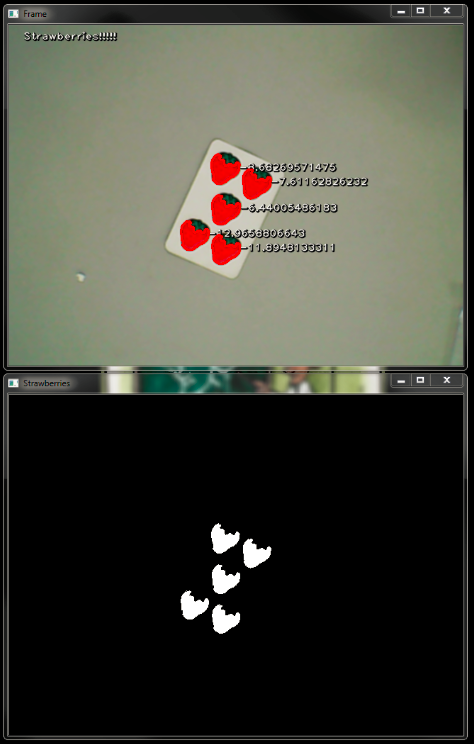
\includegraphics[height=9cm]{Abbildungen/Erdbeere01}  & 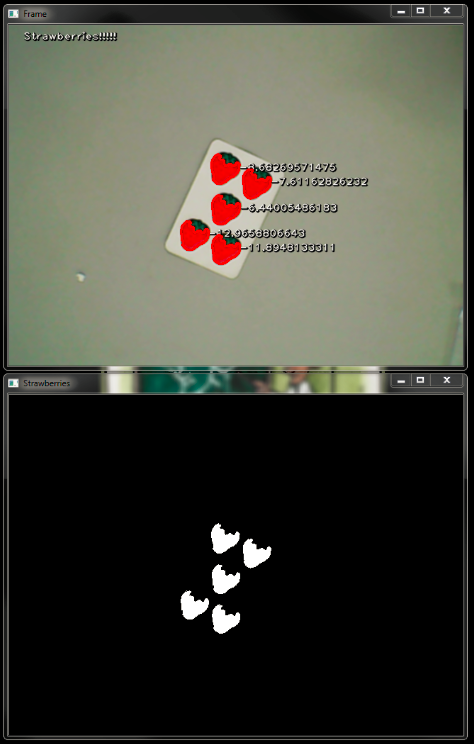
\includegraphics[height=9cm]{Abbildungen/Erdbeere01}  \\ 

\begin{center}
\begin{tabular}{cc}
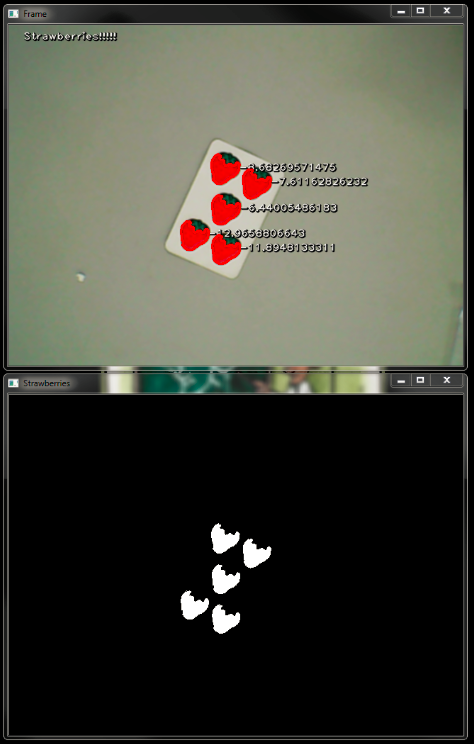
\includegraphics[height=10cm]{Abbildungen/Erdbeere01} & 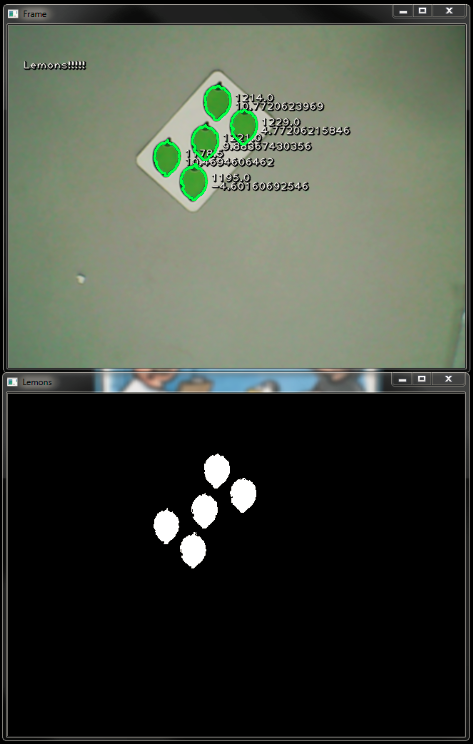
\includegraphics[height=10cm]{Abbildungen/Limonen01} \\ 
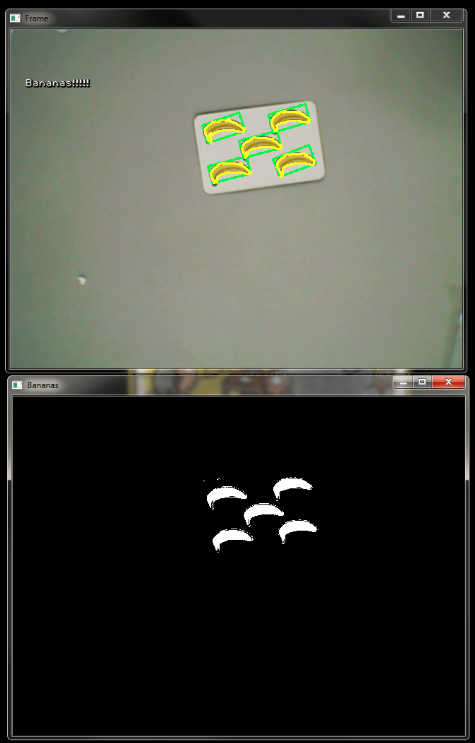
\includegraphics[height=10cm]{Abbildungen/Bananen01} & 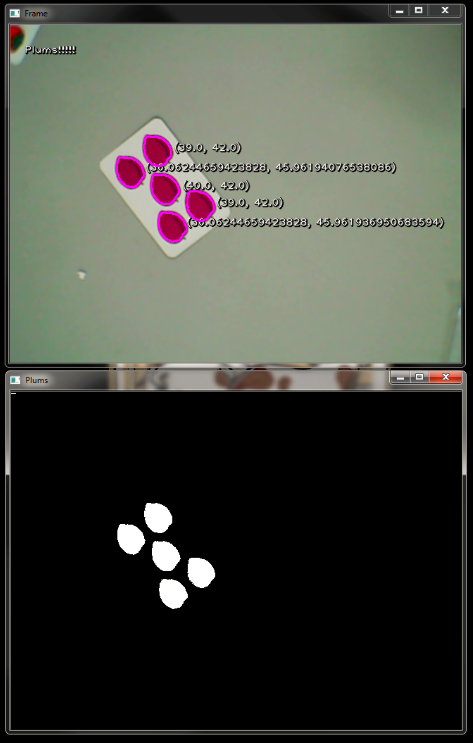
\includegraphics[height=10cm]{Abbildungen/Pflaume01} \\ 
\end{tabular}

\end{center}

\subsection{Formsegmentierung}

Wenn alle Pixel in den Farben der Früchte entdeckt und segmentiert sind, ist es notwendig die Form der gefundenen Segmente zu untersuchen. Dazu werden für jede Frucht verschiedene geometrische Verhältnisse betrachtet.

\textbf{Erdbeere}

\begin{itemize}
    \item Größe der Fläche
    \item Seitenverhältnis des kleinst - möglich umgebenden Rechteckes
    \item Verhältnis Größe der Fläche zu Größe des kleinst - möglich umgebenden Rechteckes
\end{itemize}
\lstset{language=Python}
\begin{lstlisting}[]
# Find Strawberries
    strawberries = []
    if len(strawberry_contours) > 0:
        for cnt in strawberry_contours:

            strawberry_area = cv2.contourArea(cnt)
            (x_c,y_c),radius = cv2.minEnclosingCircle(cnt)

            center = (int(x_c),int(y_c))
            radius = int(radius)
            rect = cv2.minAreaRect(cnt)
            pos, size, theta = rect
            box = cv2.cv.BoxPoints(rect)
            box = np.int0(box)
            x, y = pos
            w, h = size
            
            if 600 < strawberry_area < 1300:
                if 0.7 < h/w < 1.4:
                    area_rate = w*h/strawberry_area # 1.6
                    if 1.3 < area_rate < 1.8:
                        strawberries.append(cnt)
                        #draw_str(
                        #   frame,
                        #   (int(x)+radius, int(y)+12),
                        #    str(h/w))
                        #draw_str(
                        #   frame,
                        #   (int(x)+radius, int(y)+24),
                        #    str(strawberry_area))
                        #draw_str(
                        #   frame,
                        #   (int(x)+radius, int(y)), 
                        #   str(area_rate))
                        #cv2.drawContours(
                        #   frame,[box],0,(0,255,0),2)
\end{lstlisting}
\textbf{Pflaume}

\begin{itemize}
    \item Größe der Fläche
    \item Radius des kleinst - möglich umgebenden Kreises
    \item Seitenverhältnis des kleinst - möglich umgebenden Rechteckes
     \item Verhältnis Größe der Fläche zu Größe des kleinst - möglich umgebenden Rechteckes
\end{itemize}

\textbf{Limone}

\begin{itemize}
    \item Größe der Fläche
    \item Radius des kleinst - möglich umgebenden Kreises
    \item Seitenverhältnis des kleinst - möglich umgebenden Rechteckes
     \item Verhältnis Größe der Fläche zu Größe des kleinst - möglich umgebenden Rechteckes
\end{itemize}

\textbf{Banane}

\begin{itemize}
    \item Größe der Fläche
    \item Seitenverhältnis des kleinst - möglich umgebenden Rechteckes
    \item Längenunterschied der Seiten des kleinst - möglich umgebenden Rechteckes
    \item Verhältnis Größe der Fläche zu Größe des kleinst - möglich umgebenden Rechteckes
\end{itemize}

Die gefunden Früchte werden gezählt. Wenn genau fünf Früchte von einer Sorte gefunden werden, signalisiert ein Schriftzug auf dem Bildschirm, dass die Glocke geläutet werden muss. Auf die Glocke fertig - los!







%Ich würde sagen hier ruhig den Farbraum erklären, oder? Sollen wir ein Kapitel Hintergründe machen? Also quasi Hintergrundwissen - ?

 


